\documentclass[twoside,10pt]{article}
\usepackage{amsmath,amsfonts,amsthm,fullpage}
\usepackage{algorithm}
\usepackage{algorithmic}
\usepackage{graphicx}
\usepackage{hyperref}

\begin{document}

\title{ISYE 6740 HW 1}
\author{Mohammed Khalid Siddiqui}
\date{}

\section{Concept Questions}

\begin{enumerate}

\item In classical machine learning, Supervised learning includes both Classification and Regression
tasks whereas Unsupervised learning tends to be associated with Clustering. The primary difference between
Supervised and Unsupervised learning is that the former uses labeled data to model associations between
inputs and outputs whereas the latter does not use labeled data, instead opting to uncover associations
through similarity metrics like euclidian distance in the example of clustering. Two benefits or use-cases
of supervised learning can be to predict or forecast outputs like house prices based on a series of inputs
such as location, size, number of bedrooms and other input features as well as classify customers at risk
of churning based on a series of input data. The first task was a regression, and the second a classification.
Both are examples of supervised learning as they require input and output labels to function and attempt
to predict the output label based on the input. This serves myriad of use cases across industry. Drawbacks of
supervised learning include the need for output labels and model fitting to known data. Adding labels
such as in the case of an image dataset can be extremely time consuming. Additionally, the use of labels means
the analyst must have some idea of what they are modeling and trying to uncover. It can be harder to explore
data if you are limited to seeking a specific output which you must define. Unsupervised learning by contrast
carries the strength that allows one to explore similarities between data without explicitly defining outputs.
This focus on finding similar associations generally means that unsupervised learning may not require the training
samples in the same way supervised learning tasks do. One drawback of unsupervised learning is that unlike
supervised learning, because you aren't using labeled outputs, it may be harder to measure success via metrics like
accuracy or mean squared error etc. For this reason, unsupervised learning may be stronger suited to
exploratory data analysis tasks or creating associations of like groups without penalties for "bad" groupings.

\item Per the hint provided in the homework to use Hamming distance for the one-hot encoded version of the categorical
variables and the Google definition of (and lesson information on) Hamming distance being the number
of positions where the corresponding symbols are different, we can intuit that for any categorical variable
that has been one-hot eoncded, the Hamming distance equivalent value would be 0 if the values are the same,
and 2 if they are different, irrespective of the number of possible values available. The reason is because,
each categorical variable will only allow an observation to select one option. For example, let's assume
the second feature corresponds to 'building type' and let's say that there are n = 4 building types: "house",
"office", "apartment", "condo". Once we have one-hot encoded this feature, we will have 4 columns in the place of
the original. Each column will encode either a 1 or 0 depending on whether that value is present or not.
Going back to the example presented to us, assume the column order is the same as the list above. For those
four columns, x1 will be encoded as follows 1,0,0,0. x2 also has a building type of house and similarly, the
one-hot encoded features will appear as 1,0,0,0. If x3 were to be of type "office", the encoding would
be 0,1,0,0. Any observation can have only 1 building type. The Hamming distance for building type between x2
and x3 is 2 because two of the columns are different. The same logic can be applied to the 'city' feature.
Each observation can only have 1 city and the Hamming distance will be either 0 if agreed or 2 if disagreed.
For our numerical variable which appears to be price, we can use Euclidean distance which is
\begin{equation}
d(p,q) = \sqrt{\sum_{i=1}^{n} \left( p_i - q_i \right)^2}
\end{equation}
We will need to incorporate all three distances, the two hamming distances and the one euclidian distance
to create our clustering distance formula. This will require us to prioritize, standardize, and weight
our distances appropriately to arrive at a final distance in an reasonable manner. For the sake of simplicity,
for this problem, let's assume that city, building type, and cost are all equally important in calculating
similarity between buildings. To acheive this, we will standardize the Euclidian distance d(p,q) above
such that values are between 0 and 2. We use 2 as our upper bound because that is the maximum Hamming distance
acheivable for building type and city respectively.
I will use the following calculation to normalize the Euclidian function:
\begin{equation}
d_{\text{norm}}(x, y) = \frac{2 \cdot d(x, y)}{d_{\text{max}}}
\end{equation}
where d_max is the largest distance acheivable between building prices.
The final distance equation can act as an ensemble or combination of our three calculated distances
Hamming_buildingtype, Hamming_city, and d_norm. For a simple preliminary model, additive distance
should suffice:
\begin{equation}
d_total = Hamming_buildingtype + Hamming_city + d_norm
\end{equation}
Upon running an initial iteration of the clustering algorithm, it may be helpful to consider weighting the
different distance components or even using different transformations or formula.

\item For this problem we are comparing the functions inside the arg min function to prove their
equivalence, or specifically that given the same inputs, they will product the same outputs. The argmin
function in this instance will identify and return the value of j (the cluster a data point should be assigned to)
between 1 and k that minimizes the square of the Euclidean norm or L2 distance (As discussed in the lectures)
between the data point x_i and centroid c_j. Re-writing the Euclidean distance will be
\begin{equation}
\|x_i - c_j\|^2 = (c_j^\top c_j - 2c_j^\top x_i) + x_i^\top x_i

c_j^\top c_j - 2c_j^\top x_i

\frac{1}{2} c_j^\top c_j - c_j^\top x_i
\end{equation}
In the above we first expanded the squared L2 norm distance and re-wrote our features in vector format.
Realizing we're applying the arg min function with respect to change in j, we dropped the "constant" terms
which are identical across the two and redundant for any given data point. Lastly, knowing that the result
of the argmin function is irrespective of scale of the inputs: meaning the output of argmin(1,3) is the
same as the output of argmin(2,6) or argmin(10, 30), we divided by a factor of 2 to make the expression
equivalent to the resulting one in the homework problem.

\item K-means algorithm operates by setting initial centroids for each cluster, then identifying the points
which belong to those clusters, then updating those centroids, then identifying the points which belong to
the new clusters. This iterative process may not always converge to the "global optimal solution". I believe
in the lecture most k-means are identified as non-convex and may get trapped in local minima or converge to
local optima. This is interestingly also an issue sometimes with the gradient descent algorithm used to optimize
neural networks. In the k-means because there isn't an oscillating movement and instead a monotonic movement,
a converge is almost all but guaranteed but it won't necessarily be a globally optimal convergence. To this end,
it may be helpful to run k-means with multiple iterations using different initial centroids.

\item K-means is guaranteed to converge, if only to a local optimum not global, because there are a finite
number of k clusters ot iterate over and because the objective function, as discussed in the lectures, is
monotonically decreasing. As the objective function does not oscillate, it is guaranteed to converge to some
minimum. Due to the finite number of data points, the clusters can only update via the objective function
to a finite posisble number of combinations. Out of the three reasons provided: finite num k clusters, finite
number of data points, and monotonically decreasing objective functions, it is the objective function which
is the most compelling reason for convergence as an oscillating function could theoretically result in a loop
that continues infinitely.

\item Considering the graph provided in the question, we will first need to create an adjacency matrix,
then will we create the degree matrix. Following the degree matrix, we will then calculate the
graph Laplacian using the convenient formula L = Degree Matrix - Adjacency Matrix. Using the Graph
Laplacian, we will use the numpy library to then calculate the eigenvalues and their respective eigenvectors.
The number of 0 eigenvalues correspeonds to the number of connected components in the graph and looking
at the corresponding eigenvectors for those eigenvalues will show us which nodes belong to which connected
components because they will possess the same entries in the eigenvector. Please reference the ipynb file
for the code. Below, I'll add the relevant matrices and eigenvalues and eigenvectors printed. You'll see
the first three entries in the first eigenvector represent the first three nodes and belong to the same
connected component whereas the second eigenvector contains the last two nodes belong to the same connected
component.

\textbf{Adjacency Matrix}
\[
\begin{matrix}
0 & 1 & 1 & 0 & 0 \\
1 & 0 & 1 & 0 & 0 \\
1 & 1 & 0 & 0 & 0 \\
0 & 0 & 0 & 0 & 1 \\
0 & 0 & 0 & 1 & 1
\end{matrix}
\]

\textbf{Degree Matrix}
\[
\begin{matrix}
2 & 0 & 0 & 0 & 0 \\
0 & 2 & 0 & 0 & 0 \\
0 & 0 & 2 & 0 & 0 \\
0 & 0 & 0 & 1 & 0 \\
0 & 0 & 0 & 0 & 1
\end{matrix}
\]

\textbf{Graph Laplacian: D - A}
\[
\begin{matrix}
2 & -1 & -1 & 0 & 0 \\
-1 & 2 & -1 & 0 & 0 \\
-1 & -1 & 2 & 0 & 0 \\
0 & 0 & 0 & 1 & -1 \\
0 & 0 & 0 & -1 & 1
\end{matrix}
\]

\textbf{Eigenvalues}
\[
\begin{matrix}
0 & 0 & 2 & 3 & 3
\end{matrix}
\]

\textbf{Relevant Eigenvectors (correspond to eigenvalues = 0)}
\[
\begin{matrix}
-0.57735027 & 0  \\
-0.57735027 & 0  \\
-0.57735027 & 0  \\
0 & 0.70710678  \\
0 & 0.70710678
\end{matrix}
\]
\end{enumerate}

\section{Math of k-means Clustering}

\begin{enumerate}

\item :et's look at the equations provided before we start to answer the questions.
\begin{equation}
J =\sum_{i=1}^m\sum_{j=1}^k r^{ij} \|\text x^i-\mu^j\|^2,
\label{J_def}
\end{equation}
$$\mu^j=\frac{\sum_i r^{ij} \text x^i}{\sum_i r^{ij}}.$$

The first equation states that the k-means function seeks to minimize the distortion J by summing up
the squared euclidian distance for each data point from its respective centroid.The r_ij term ensures that
we do not take the distance of a datapoint from a centroid other than its own in our calculation. The final
derived equation below states that the centroid Mu for a given cluster j that minimizes the distortion
function J is the sum of all data points in that cluster divided by the total number of data points in that
cluster, which is essentially the average of all the points in that cluster j. Similarly to a previous concept
question, we can first expand the squared Euclidian distance to write in a format we are accustomed to. To
find critical points such as minimum or maximum, we will then take the derivative with respect to our variable
of interest (in this case the centroid Mu_j which we are trying to optimize to minimize the distortion function
J). Once we set the derivative to 0, we can solve for the value of centroid Mu_j.

\[
\| x_i - \mu_j \|^2 = (x_i - \mu_j)^T(x_i - \mu_j)
\]

\[
\frac{\partial J}{\partial \mu_j} = \sum_{i=1}^{m} r_{ij} \cdot 2(\mu_j - x_i) = 0
\]

\[
\mu_j = \frac{\sum_{i=1}^{m} r_{ij} x_i}{\sum_{i=1}^{m} r_{ij}}
\]

In the final steps, Mu_j can be pulled out of the sum and treated as a constant as it doesn't vary with i
like the r_ij term does, allowing us to simply expand the summation terms and divide to isolate Mu_j on the
left side of the equation.

\item The variable r_ij is 1 when the datapoint x_i belongs to the jth cluster and 0 when it doesn't as
mentioned in the first part of the section. If we have a fixed centroid and need to determine whether
r_ij should be 1 or 0, we need to find the closest centroid to that data point and only assign 1 when
that is true. To accomplish this, for a given point x_i, we will need to traverse all centroids Mu_j for all
j clusters and then find the minimum distance (in our case the squared euclidian distance) between the point
and the centroid and return 1 for that combination. As in the previous concept section and lectures, we can use the
concept of argmin function to help accomplish this. Mathematically, our function will appear as:

\begin{equation}
\[
r_{ij} =
\begin{cases}
1 & \text{if } j = \arg \min_{j'} \| x_i - \mu_{j'} \|^2 \\
0 & \text{otherwise}
\end{cases}
\]
\end{equation}

This will minimize the distortion function j as the r_ij values are now set appropriately.

\item We'll now accomplish part 1 and 2 for the situation where instead of euclidean distance,
we use the Mahalnobis distance in minimizing the cost-function.
\[
J =\sum_{i=1}^m\sum_{j=1}^k r^{ij} (\text x^i-\mu^j)^T \Sigma  (\text x^i-\mu^j),
\]

Per the source I've linked below, the Mahalnobis distance is the relative distance of point x_i, from the center
of mass y (in our case, the centroid Mu_j). The transpose vector of x_i - Mu_j is multiplied by the
inverse of the covariance matrix multipled by x_i - Mu_j. This essentially introduces a normalization
component. Additionally, like our squared euclidian distance in the prior problem, we have the squared
Mahalanobis distance. The steps we take will be identical to those we took to solve for the
respective Mu_j and r_ij of the euclidian squared distance. However, now we simply have an additional
covariance term to be concerned with. I'll skip ahead to the parts that will look different.
\[
\frac{\partial J}{\partial \boldsymbol{\mu}_j} = -2 \sum_{i=1}^{m} r_{ij} \Sigma (\mathbf{x}_i - \boldsymbol{\mu}_j)
\]

\[
-2 \sum_{i=1}^{m} r_{ij} \Sigma (\mathbf{x}_i - \boldsymbol{\mu}_j) = 0
\]

\[
\sum_{i=1}^{m} r_{ij} \Sigma \mathbf{x}_i = \sum_{i=1}^{m} r_{ij} \Sigma \boldsymbol{\mu}_j
\]

\[
\boldsymbol{\mu}_j \sum_{i=1}^{m} r_{ij} = \sum_{i=1}^{m} r_{ij} \mathbf{x}_i
\]

\[
\boldsymbol{\mu}_j = \frac{\sum_{i=1}^{m} r_{ij} \mathbf{x}_i}{\sum_{i=1}^{m} r_{ij}}
\]

Note, that we 'cancelled' out the covariance definite matrix present on both sides. Also note how the
optimal centroid M_j for cluster j looks identical to the one from the l2-norm squared, as the average
of the data points within the cluster. For the cluster assignment solving for r_ij, we'll follow the same
logic we did for the l2_norm squared distance. Namely, we realize we are setting r_ij to 1 where
the distance between a point and cluster is the minimum for all given clusters. We will simply replace
the distance function to the Mahalanobis distance squared formula provided in the assignment.

\[
r_{ij} = \begin{cases}
1 & \text{if } j = \arg \min_{j'} \; (\mathbf{x}_i - \boldsymbol{\mu}_{j'})^T \Sigma (\mathbf{x}_i - \boldsymbol{\mu}_{j'}) \\
0 & \text{otherwise}
\end{cases}
\]


Source used to understand Mahalanobis distance: https://math.stackexchange.com/questions/428064/distance-of-a-test-point-from-the-center-of-an-ellipsoid
Another source: https://www.statisticshowto.com/mahalanobis-distance/
Another source: https://mccormickml.com/2014/07/22/mahalanobis-distance/
\end{enumerate}

\section{Image Compression Using Clustering}

Third image source: https://commons.wikimedia.org/wiki/File:Greycat.jpg

The code for the Image Compression is in the Jupyter Notebook, as are the output images and original images.
I originally wrote a k-means algorithm which would randomly re-assign centroid location for empty clusters and this
performed well with respect to visual appearance of the rendered images. To bring my submission more in line
with the requirements for the assignment, I implemented a change such that during a given iteration, any empty
cluster was dropped. For low number k, this was't an issue, however, for k = 16 and k = 32, all three images
exhibit significant drops, with final number of clusters anywhere from 11 to 25 respectively. I could visually
tell that the image was not as crisp as the original nor the rendered images with re-assigned clusters. Additionally,
the time it took to run my function in both cases was roughly the same about 2 minutes to 3 minutes for the
football image depending on the set of random numbers I used. Later, I added a seed of 123 for reproducibility.

Additionally, although I originally implemented a loop to calculate the distance and assign points to centroids,
I then used numpy calculations before switching entirely to using the lin.alg.norm built-in function to help
calculate the l2_norm squared or euclidian squared distance. I've commented out the originals to show the implementation.

For each k, I ran 5 runs and selected the best run by minimizing the within cluster sum of squares metric.
Per Datanovia (source link below), the within cluster sum of squares is a method capturing within cluster variance
and captures the "compactness" of clusters. To calculate, the squared difference of the distance between
data points and centroids are calculated and then summed for all clusters. A lower WCSS indicates that points
tend to be closer to their centroids and are therefore better fit. In our runs, the iterations which on average
had the lowest WCSS or the best fitting clusters were selected for each k. The kmeans package in R allows you
to set the number of initial starts parameter nstart which is highly recommended. You can do 25, 50 or many more
runs. In doing so, you may develop more stable results by selecting the variant with the lowest WCSS.

The higher the number of centroids k, the longer the algorithm took to run. For the football image, the best
run for k = 2 took 0.36 seconds, while the best run for k = 32 took 15.15 total seconds. This makes
sense as increasing the number of k makes running the algorithm computationally expensive. Similarly, the number
of iterations kmeans went through before converging also increased as the k did. For the football image,
when k = 2, I only need 7 iterations for the best run, whereas when k = 32, I required 42 iterations for the best
run. This makes sense as having more clusters would take longer to converge.

I returned multiple data points in my kmeans function which I printed out as part of the run_k_means_and_visualize
function. These included the length of the best iteration, k, number of centroids, best initialized centroids,
and the number of iterations for each run as well as the best image itself. You can see the rendered images
for each specified k as well as the three original images below.

As for finding the best k for this specific image compression issue, this depends entirely on your goals. The lower
the number of clusters k, the more compressed the image will be and the less time it will take to run the algorithm.
However, in doing so, the visual representation will not be as crisp or clear as a higher k rendered image. It is
important to determine what the situation calls for in determining how much to compress the image. In this instance,
k = 32 provided the best rendered image though it may take up more space than the lower k images. Additionally,
at 15 seconds a run, it didn't take too long. However, in other situations, determining the optimal number of clusters
is wholly determined by the problem. One method used to determine optimal k is the elbow method. where one may
plot the WCSS for different values of k and then find the "elbow" or sharp flattening of the curve which will
correspond to an optimal k. Another method is to simply use domain knowledge or visually plot the data (when possible)
to highlight existing clusters. There are other methods such as Silhouette analysis etc. For image compression,
a visual cue along with examing tradeoff between visual acuity, size, and time to compute + render are the
tradeoffs we would examine as the image will become more crisp as k increases.

\subsection{Football}
\begin{figure}
    \centering
    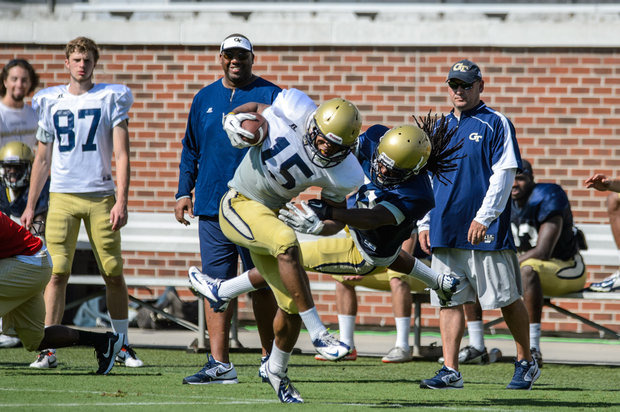
\includegraphics{c/users/moham/pycharmprojects/hw1_isye_6740/data/football}
    \caption{Original}
    \label{fig:football}
\end{figure}

\begin{figure}
    \centering
    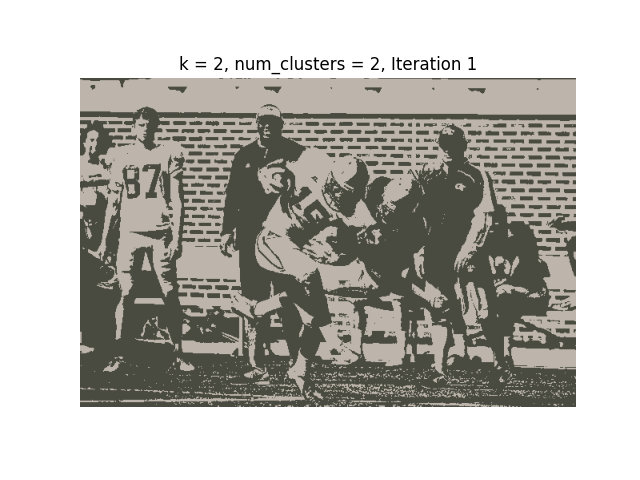
\includegraphics{C:\Users\moham\PycharmProjects\HW1_ISYE_6740\outputs\football_2}
    \caption{K = 2}
    \label{fig:football_2}
\end{figure}

\begin{figure}
    \centering
    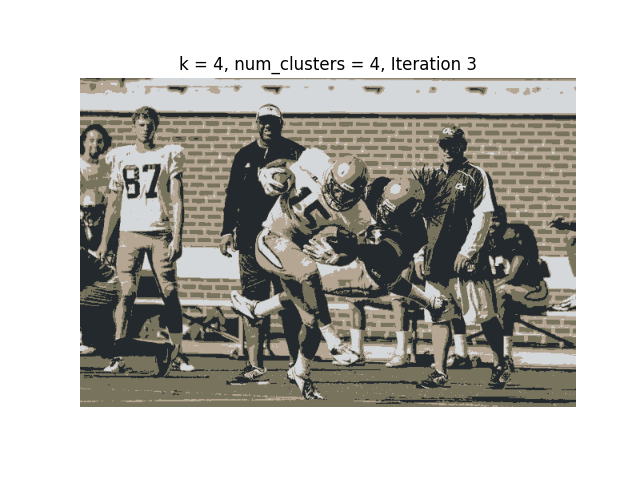
\includegraphics{C:\Users\moham\PycharmProjects\HW1_ISYE_6740\outputs\football_4}
    \caption{K = 4}
    \label{fig:football_4}
\end{figure}

\begin{figure}
    \centering
    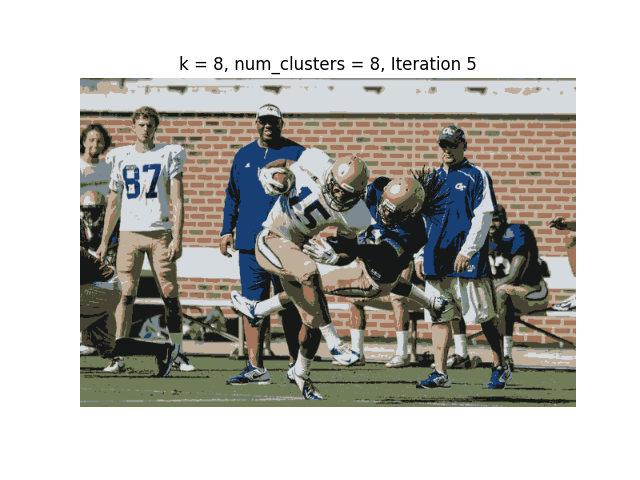
\includegraphics{C:\Users\moham\PycharmProjects\HW1_ISYE_6740\outputs\football_8}
    \caption{K = 8}
    \label{fig:football_8}
\end{figure}

\begin{figure}
    \centering
    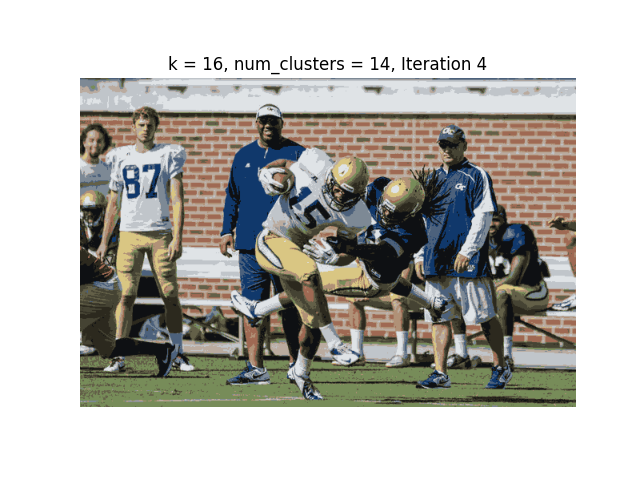
\includegraphics{C:\Users\moham\PycharmProjects\HW1_ISYE_6740\outputs\football_16}
    \caption{K = 16}
    \label{fig:football_16}
\end{figure}


\begin{figure}
    \centering
    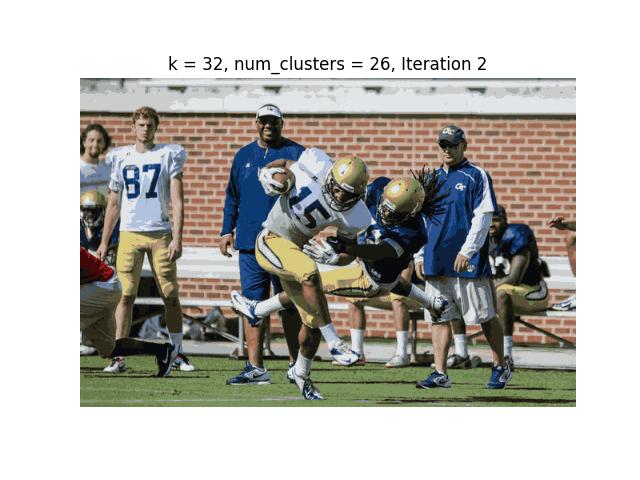
\includegraphics{C:\Users\moham\PycharmProjects\HW1_ISYE_6740\outputs\football_32}
    \caption{K = 32}
    \label{fig:football_32}
\end{figure}

\subsection{Cat}
\begin{figure}
    \centering
    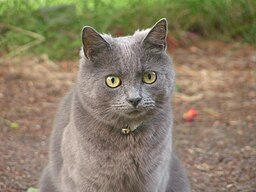
\includegraphics{C:\Users\moham\PycharmProjects\HW1_ISYE_6740\data\256px-Greycat}
    \caption{Original}
    \label{fig:256px-greycat}
\end{figure}

\begin{figure}
    \centering
    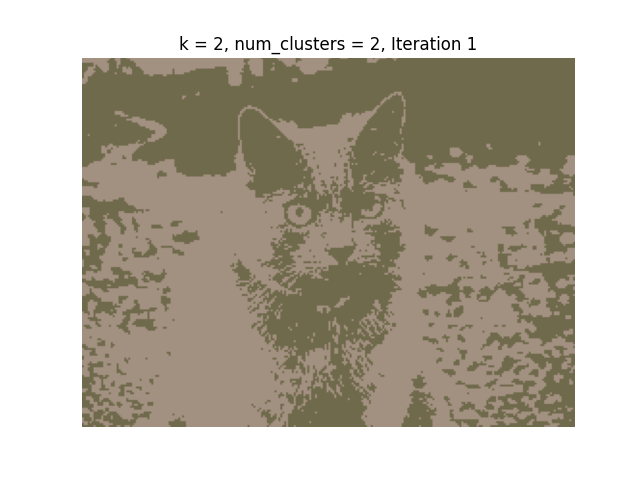
\includegraphics{C:\Users\moham\PycharmProjects\HW1_ISYE_6740\outputs\256px-Greycat_2}
    \caption{K = 2}
    \label{fig:256px-greycat_2}
\end{figure}

\begin{figure}
    \centering
    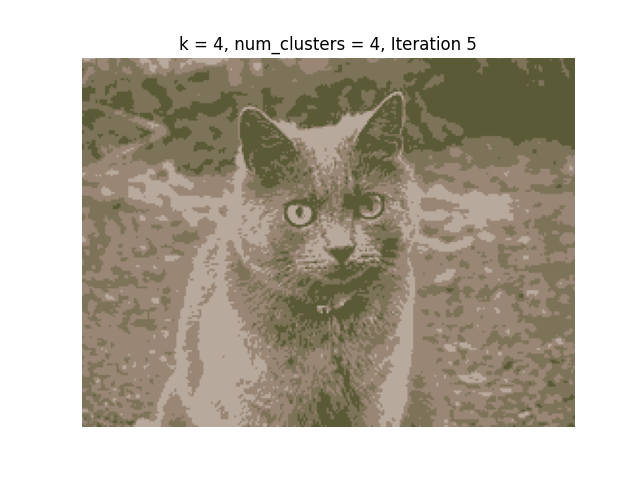
\includegraphics{C:\Users\moham\PycharmProjects\HW1_ISYE_6740\outputs\256px-Greycat_4}
    \caption{K = 4}
    \label{fig:256px-greycat_4}
\end{figure}

\begin{figure}
    \centering
    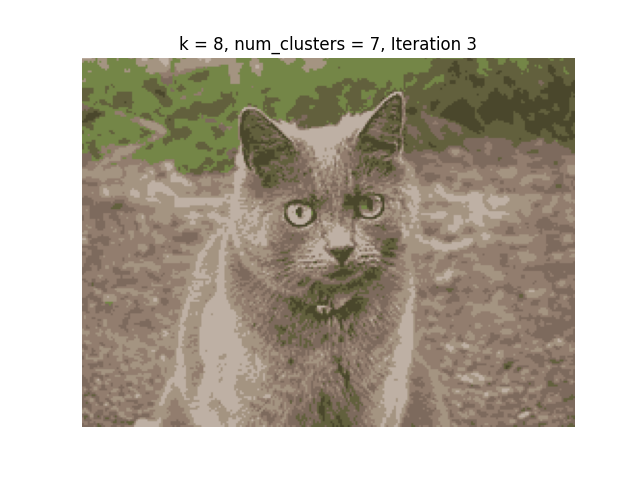
\includegraphics{C:\Users\moham\PycharmProjects\HW1_ISYE_6740\outputs\256px-Greycat_8}
    \caption{K = 8}
    \label{fig:256px-greycat_8}
\end{figure}

\begin{figure}
    \centering
    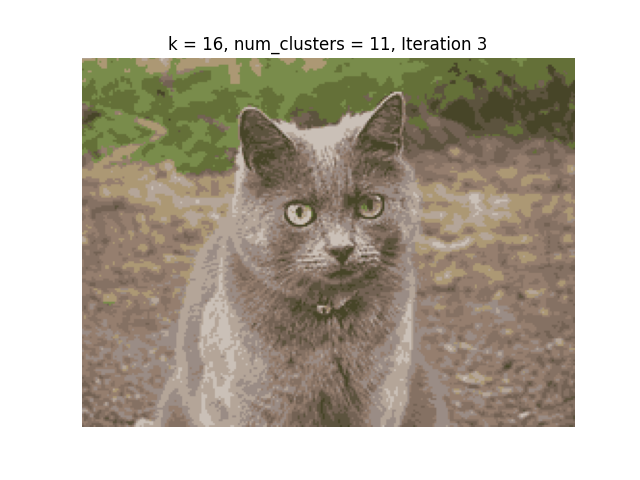
\includegraphics{C:\Users\moham\PycharmProjects\HW1_ISYE_6740\outputs\256px-Greycat_16}
    \caption{K = 16}
    \label{fig:256px-greycat_16}
\end{figure}

\begin{figure}
    \centering
    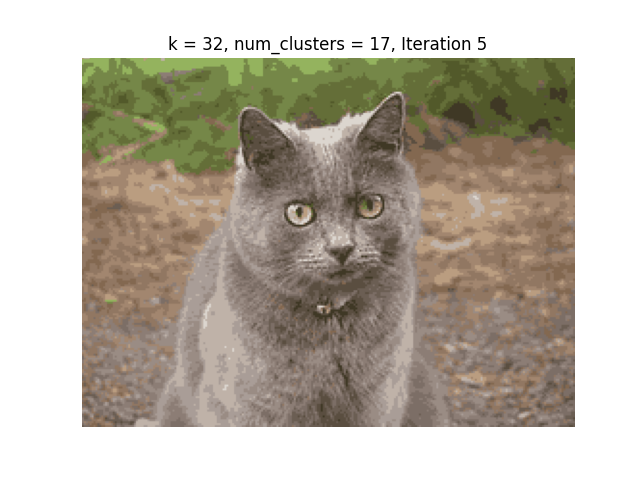
\includegraphics{C:\Users\moham\PycharmProjects\HW1_ISYE_6740\outputs\256px-Greycat_32}
    \caption{K = 32}
    \label{fig:256px-greycat_32}
\end{figure}


\subsection{Coastal Abstract}

\begin{figure}
    \centering
    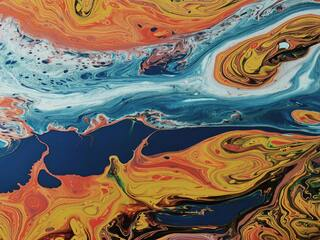
\includegraphics{C:\Users\moham\PycharmProjects\HW1_ISYE_6740\data\coastal-abstract}
    \caption{Original}
    \label{fig:coastal-abstract}
\end{figure}

\begin{figure}
    \centering
    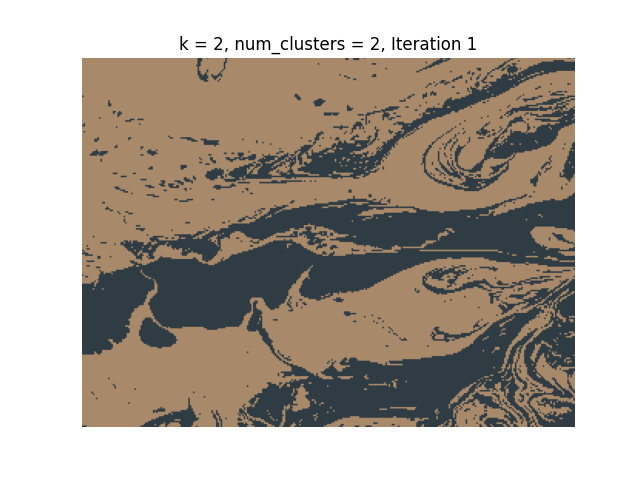
\includegraphics{C:\Users\moham\PycharmProjects\HW1_ISYE_6740\outputs\coastal-abstract_2}
    \caption{K = 2}
    \label{fig:coastal-abstract_2}
\end{figure}

\begin{figure}
    \centering
    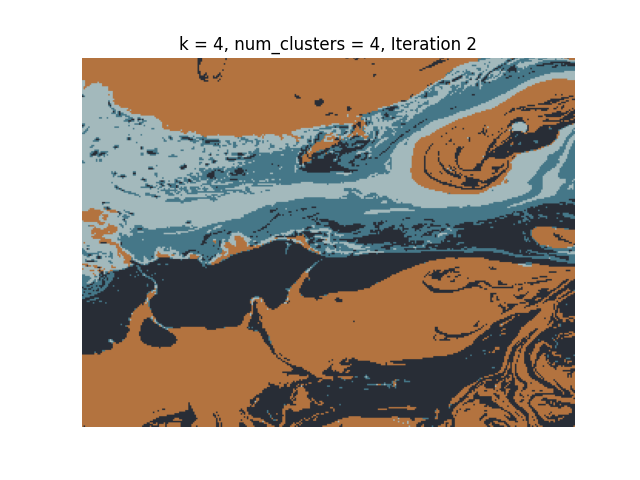
\includegraphics{C:\Users\moham\PycharmProjects\HW1_ISYE_6740\outputs\coastal-abstract_4}
    \caption{K = 4}
    \label{fig:coastal-abstract_4}
\end{figure}

\begin{figure}
    \centering
    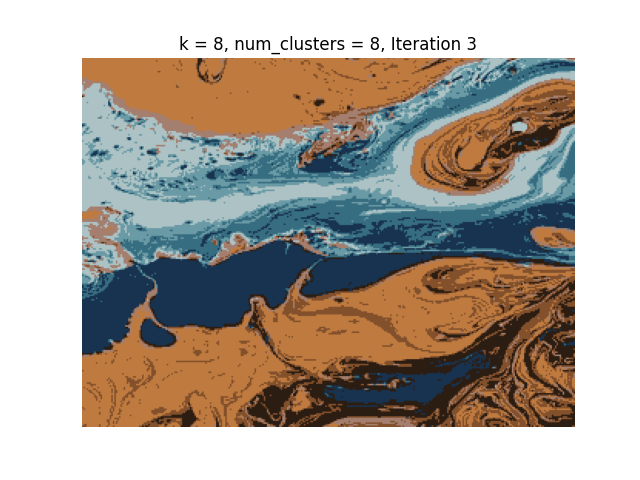
\includegraphics{C:\Users\moham\PycharmProjects\HW1_ISYE_6740\outputs\coastal-abstract_8}
    \caption{K = 8}
    \label{fig:coastal-abstract_8}
\end{figure}

\begin{figure}
    \centering
    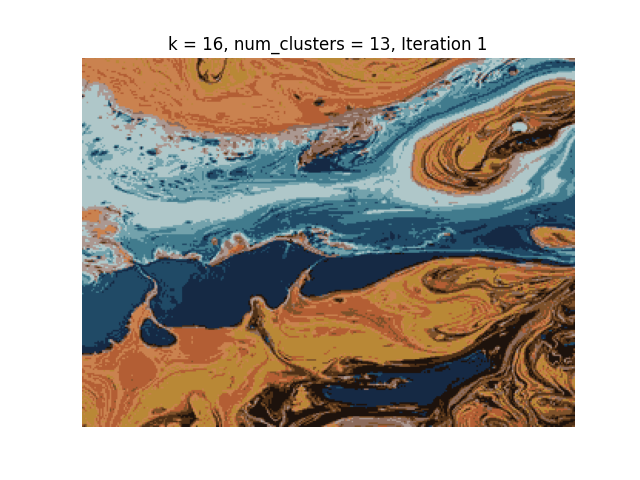
\includegraphics{C:\Users\moham\PycharmProjects\HW1_ISYE_6740\outputs\coastal-abstract_16}
    \caption{K = 16}
    \label{fig:coastal-abstract_16}
\end{figure}

\begin{figure}
    \centering
    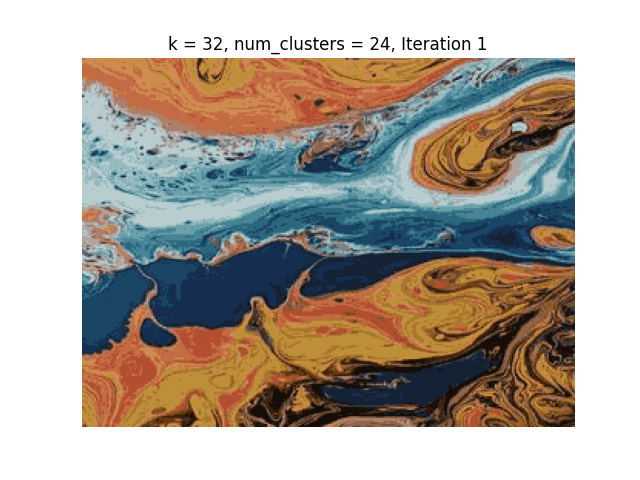
\includegraphics{C:\Users\moham\PycharmProjects\HW1_ISYE_6740\outputs\coastal-abstract_32}
    \caption{K = 32}
    \label{fig:coastal-abstract_32}
\end{figure}

\subsection{Sources}

\begin{enumerate}
\item https://www.datanovia.com/en/lessons/k-means-clustering-in-r-algorith-and-practical-examples/
\item https://www.geeksforgeeks.org/find-a-matrix-or-vector-norm-using-numpy/#
\item https://www.w3schools.com/python/numpy/numpy_creating_arrays.asp
\item https://numpy.org/doc/stable/reference/generated/numpy.zeros.html
\item https://numpy.org/devdocs/reference/constants.html#numpy.newaxis
\item https://note.nkmk.me/en/python-opencv-bgr-rgb-cvtcolor/
\item https://stackoverflow.com/questions/49434754/how-does-the-pyplot-imshow-function-work
\item https://www.geeksforgeeks.org/ml-determine-the-optimal-value-of-k-in-k-means-clustering/

\end{enumerate}

\subsection{Steps Taken for Algorithm}
Steps Taken:
- convert images into pixel color representations
- define the number of clusters
- set the initial position of each cluster randomly (you are going to run this multiple times)
- use the l2-norm squared distance formula for each pixel to assign a cluster
- update the clusters
- repeat assignment until convergence

\section{MNIST Dataset Clustering}

Steps I took:
- load in the MNIST file
- only maintain the train data set (per instructions)
- preprocess per instructions
- write (or import) the k-means with eucldiean squared distance
- write (or import) the k-means with manhattan squared distance
- calculate clusters for each image/data point
- assign class (from labeled y data) to each cluster based on which class is most common for a given cluster
- calculate purity score for both kmeans runs for each cluster as well as average purity score

\subsection{Results and Discussion}
Please reference the added Jupyter notebook for code and direct output. I used the pyclustering library
implementation of kmeans so that I could easily use both Manhattan and squared l2norm distance metrics.
Additionally, I implemented the kmeans++ methodolgy of setting initial centroids to avoid needing to run each
algorithm multiple times and choose the run with the lowest WCSS as I did for section 3. Following the steps
I took outlined in the above (standardizing, dropping test sets, assigning clusters, finding the majority
labels, anc calculating purity score as shown below), I was able to obtain average purity score of roughly 58.28
percent when using squared euclidean as the distance metric and 51.69 when using Manhattan distance as the distance
metric. This suggests that the squared euclidean distance metric captures the MNIST data structure more effectively
as it is more sensitive to large differences in distances between data points than manhattan distance.
\[
\mbox{purity}_i = \frac{\mbox{corrected assigned samples}_i}{\mbox{size of cluster}_i}
\]
Below are the individual purity scores and assigned label for each cluster for the Euclidean Squared distance
run of the K-Means algorithm


\begin{tabular}{|c|c|c|}
\hline
\textbf{Cluster} & \textbf{Assigned Label} & \textbf{Purity Score} \\
\hline
0 & 1 & 0.5902 \\
\hline
1 & 0 & 0.9385 \\
\hline
2 & 3 & 0.5310 \\
\hline
3 & 5 & 0.3058 \\
\hline
4 & 6 & 0.8723 \\
\hline
5 & 1 & 0.6471 \\
\hline
6 & 4 & 0.3585 \\
\hline
7 & 8 & 0.6194 \\
\hline
8 & 2 & 0.9177 \\
\hline
9 & 7 & 0.4367 \\
\hline
\end{tabular}

Below are the individual purity scores and assigned label for each cluster for the Manhattan distance
run of the K-Means algorithm.


\begin{table}[h!]
\centering
\begin{tabular}{|c|c|c|}
\hline
\textbf{Cluster} & \textbf{Assigned Label} & \textbf{Purity Score} \\
\hline
0 & 8 & 0.5693 \\
1 & 8 & 0.4366 \\
2 & 1 & 0.3586 \\
3 & 7 & 0.3841 \\
4 & 6 & 0.8728 \\
5 & 0 & 0.9410 \\
6 & 3 & 0.5966 \\
7 & 2 & 0.9603 \\
8 & 4 & 0.3948 \\
9 & 0 & 0.8901 \\
\hline
\end{tabular}
\caption{Cluster Assignments and Purity Scores}
\label{tab:cluster_purity}
\end{table}

\susection{Sources}
\begin{enumerate}
\item https://www.kaggle.com/code/arushchillar/kmeans-clustering-using-different-distance-metrics
\item https://yann.lecun.com/exdb/mnist/
\item https://stackoverflow.com/questions/76246578/module-numpy-has-no-attribute-warnings
\item https://pyclustering.github.io/docs/0.8.2/html/da/d22/classpyclustering_1_1cluster_1_1kmeans_1_1kmeans.html
\item https://numpy.org/doc/stable/reference/generated/numpy.bincount.html
\end{enumerate}
\end{document}